\chapter{Additional Notes}
\section{Source code}
The source code is well developed both in the flutter app and the server. The general structure of the code follows the MVC pattern as stated in the DD.\newline
Some parts of the backend could be better documented but nothing too serious, nevertheless the client side is very well documented.

\section{User Interface Concerns}
During the testing of the User Interface of the flutter application we encountered some UI bad behaviours.\newline
We make this evident just because on the ITD it was stated that the development of the application was focused on the user experience.

\begin{itemize}
	\item There are some pop up messages which don't tell nothing about what is happening. For example, when an operator calls a customer, an empty pop up is shown.
	\vspace{0.5cm}
	\begin{figure}[H]
		\centering
		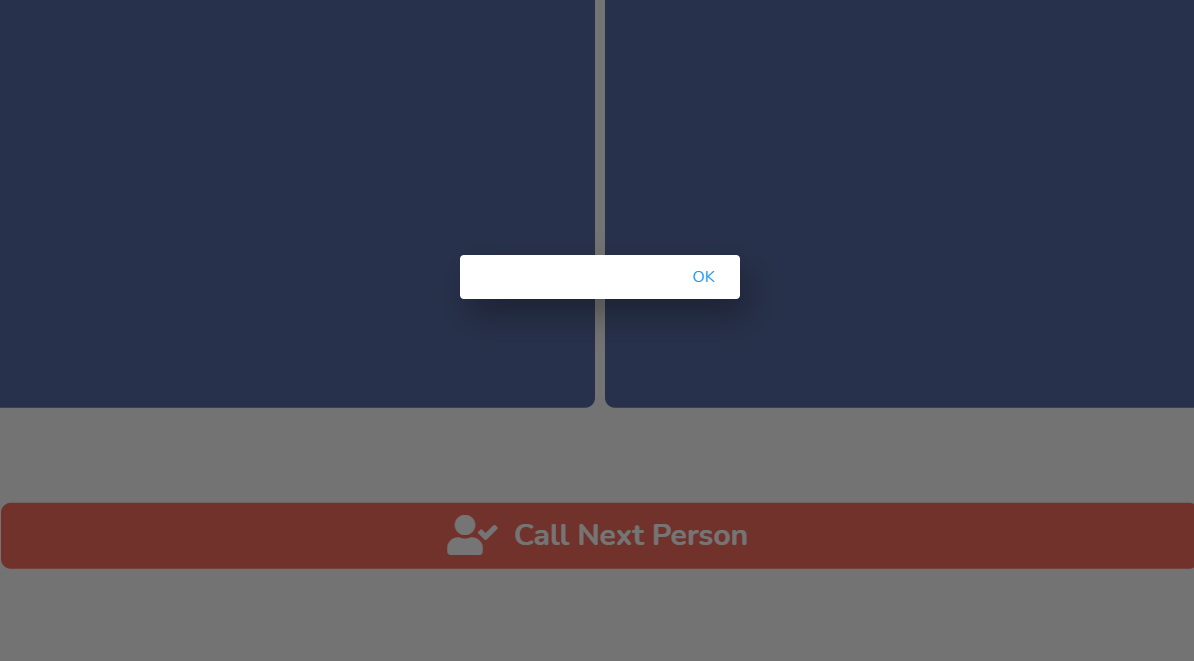
\includegraphics[width=.7\textwidth]{screen1}
	\end{figure}
	\clearpage
	\item When a customer is called, the app shows to him an alert telling that he was called. This happens every 10 seconds causing the stacking of several messages.
	
	\vspace{0.5cm}
	\begin{minipage}{.5\textwidth}
		\centering
		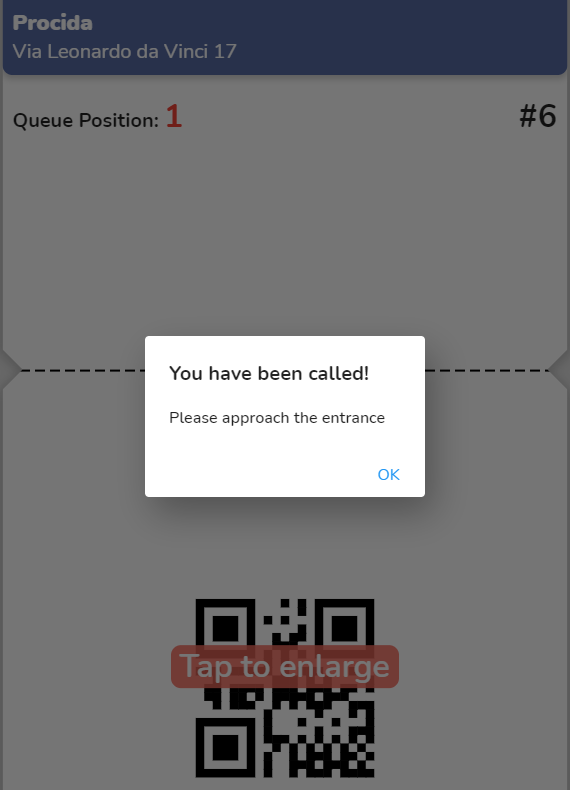
\includegraphics[width=.6\textwidth]{screen3}
		\captionsetup{type=figure}
	\end{minipage}%
	\begin{minipage}{.5\textwidth}
		\centering
		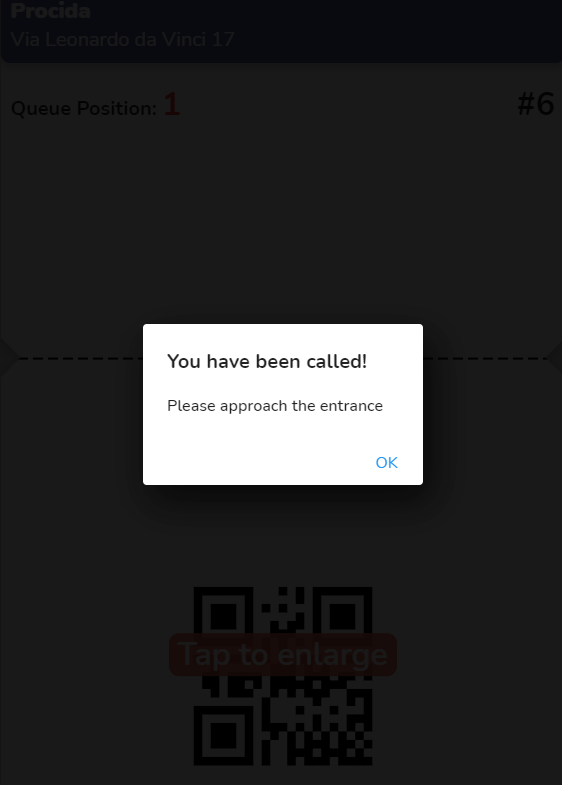
\includegraphics[width=.6\textwidth]{screen2}
		\captionsetup{type=figure}
	\end{minipage}
\end{itemize}